\documentclass{article}

\usepackage[utf8]{inputenc}
\usepackage{amsmath}
\usepackage{amssymb}
\usepackage{amsthm}
\usepackage{ifthen}
\usepackage{xparse}
%\usepackage{tikz}
%\usetikzlibrary{decorations.fractals}
\usepackage{graphicx}

\newcommand{\sizedescriptor}[2]
{
\ifthenelse{\equal{#1}{0}}{}{
\ifthenelse{\equal{#1}{1}}{\big}{
\ifthenelse{\equal{#1}{2}}{\Big}{
\ifthenelse{\equal{#1}{3}}{\bigg}{
\ifthenelse{\equal{#1}{4}}{\Bigg}{
#2}}}}}
}

\NewDocumentCommand{\set}
{O{auto} m G{\empty}}
{\sizedescriptor{#1}{\left}\{ {#2} \ifthenelse{\equal{#3}{}}{}{ \; \sizedescriptor{#1}{\middle}| \; {#3}} \sizedescriptor{#1}{\right}\}}

\newcommand{\pow}{\mathcal{P}}

\newcommand{\all}[1]{\forall #1 .\,}
\newcommand{\some}[1]{\exists #1 .\,}
\newcommand{\exactlyone}[1]{\exists{!} #1 .\,}
\newcommand{\lam}[1]{\lambda #1 .\,}
\newcommand{\that}[1]{\iota #1 .\,}

\usepackage[slovene]{babel}
\newcommand{\lthen}{\Rightarrow}
\newcommand{\two}{\mathbf{2}}
\newcommand{\true}{\top}
\newcommand{\false}{\bot}

\newcommand{\NN}{\mathbb{N}}
\newcommand{\ZZ}{\mathbb{Z}}
\newcommand{\QQ}{\mathbb{Q}}
\newcommand{\RR}{\mathbb{R}}

%%%%%%%%%%%%%%%%%%%%%%%%%%%%%%%%%%%%%%%%%%%%%%%%%%%%%%%%%%%%%%%%%%%%%%%%%%%%%%%%%%%%%%%%%%%%%%%%%%%%%%%%%%%%%%%%%%%%%%%
%%%  Commands
%%%%%%%%%%%%%%%%%%%%%%%%%%%%%%%%%%%%%%%%%%%%%%%%%%%%%%%%%%%%%%%%%%%%%%%%%%%%%%%%%%%%%%%%%%%%%%%%%%%%%%%%%%%%%%%%%%%%%%


%%%%%%%%%%%%%%%%%%%%%%%%%%%%%%%%%%%%%%%%%%%%%%%%%%%%%%%%%%%%%
%%%  Theorems etc.
%%%%%%%%%%%%%%%%%%%%%%%%%%%%%%%%%%%%%%%%%%%%%%%%%%%%%%%%%%%%%
{
\theoremstyle{theorem}
\newtheorem{izrek}{Izrek}[chapter]
\newtheorem{lema}[izrek]{Lema}
\newtheorem{trditev}[izrek]{Trditev}
\newtheorem{posledica}[izrek]{Posledica}
\newtheorem{pravilo}[izrek]{Pravilo}
}

{
\theoremstyle{definition}
\newtheorem{definicija}[izrek]{Definicija}
\newtheorem{opomba}[izrek]{Opomba}
\newtheorem{primer}[izrek]{Primer}
\newtheorem{zgled}[izrek]{Zgled}
\newtheorem{naloga}[izrek]{Naloga}
}


%%%%%%  Proofs
%%%%%%%%%%%%%%%%%%%%%%%%%%%%%%%%%%%%%%%%%%%%%%%%%%%%%%%%%%%%%
% Za dokaze uporabimo amsmath proof, sicer ne deluje \qedhere.


%%%%%%  Auxiliary
%%%%%%%%%%%%%%%%%%%%%%%%%%%%%%%%%%%%%%%%%%%%%%%%%%%%%%%%%%%%%
\newcommand{\sizedescriptor}[2]
{
\ifthenelse{\equal{#1}{0}}{}{
\ifthenelse{\equal{#1}{1}}{\big}{
\ifthenelse{\equal{#1}{2}}{\Big}{
\ifthenelse{\equal{#1}{3}}{\bigg}{
\ifthenelse{\equal{#1}{4}}{\Bigg}{
#2}}}}}
}

\newcommand{\someref}{{\small\textcolor{blue}{[\textbf{ref.}]}}}
\newcommand{\intermission}{\bigskip\medskip}
\newcommand{\ltc}[1]{$\backslash$\texttt{#1}}  % LaTeX command
\newcommand{\nls}[1]{``\textit{#1}''}  % sentence in a natural language

%%%%%%  Logical Quantifiers, λ- and ι-Expressions
%%%%%%%%%%%%%%%%%%%%%%%%%%%%%%%%%%%%%%%%%%%%%%%%%%%%%%%%%%%%%

\newcommand{\all}[1]{\forall #1 .\,}
\newcommand{\some}[1]{\exists #1 .\,}
\newcommand{\exactlyone}[1]{\exists{!} #1 .\,}
\newcommand{\lam}[1]{\lambda #1 .\,}
\newcommand{\that}[1]{\iota #1 .\,}

%%%%%%  Logic
%%%%%%%%%%%%%%%%%%%%%%%%%%%%%%%%%%%%%%%%%%%%%%%%%%%%%%%%%%%%%
\newcommand{\tvs}{\Omega}  % set of truth values
\newcommand{\true}{\top}  % truth
\newcommand{\false}{\bot}  % falsehood
\newcommand{\etrue}{\boldsymbol{\top}}  % emphasized truth
\newcommand{\efalse}{\boldsymbol{\bot}}  % emphasized falsehood
\newcommand{\impl}{\Rightarrow}  % implication sign
\newcommand{\revimpl}{\Leftarrow}  % reverse implication sign
\newcommand{\lequ}{\Leftrightarrow}  % equivalence sign
\newcommand{\xor}{\mathbin{\veebar}}  % exclusive disjunction sign
\newcommand{\shf}{\mathbin{\uparrow}}  % Sheffer connective
\newcommand{\luk}{\mathbin{\downarrow}}  % Łukasiewicz connective


%%%%%%  Sets
%%%%%%%%%%%%%%%%%%%%%%%%%%%%%%%%%%%%%%%%%%%%%%%%%%%%%%%%%%%%%
%  \set{1, 2, 3}         ->  {1, 2, 3}
%  \set{a \in X}{a < 1}  ->  {a ∈ X | a < 1}
\NewDocumentCommand{\set}
{O{auto} m G{\empty}}
{\sizedescriptor{#1}{\left}\{ {#2} \ifthenelse{\equal{#3}{}}{}{ \; \sizedescriptor{#1}{\middle}| \; {#3}} \sizedescriptor{#1}{\right}\}}
%\newcommand{\vsubset}{\Mapstochar\cap}
%\newcommand{\finseq}[1]{{#1}^*}
\newcommand{\pst}{\mathcal{P}}
\renewcommand{\complement}[1]{{#1}^C}


%%%%%%  Number Sets, Intervals
%%%%%%%%%%%%%%%%%%%%%%%%%%%%%%%%%%%%%%%%%%%%%%%%%%%%%%%%%%%%%
\newcommand{\NN}{\mathbb{N}}
\newcommand{\ZZ}{\mathbb{Z}}
\newcommand{\QQ}{\mathbb{Q}}
\newcommand{\RR}{\mathbb{R}}
\newcommand{\CC}{\mathbb{C}}
\newcommand{\intoo}[3][\RR]{{#1}_{(#2, #3)}}
\newcommand{\intcc}[3][\RR]{{#1}_{[#2, #3]}}
\newcommand{\intoc}[3][\RR]{{#1}_{(#2, #3]}}
\newcommand{\intco}[3][\RR]{{#1}_{[#2, #3)}}


%%%%%%  Maps and Relations
%%%%%%%%%%%%%%%%%%%%%%%%%%%%%%%%%%%%%%%%%%%%%%%%%%%%%%%%%%%%%
\newcommand{\id}[1][]{\mathrm{id}_{#1}}  % identity map
\newcommand{\argbox}{{\;\!\fbox{\phantom{M}}\;\!}}  % box for a function argument
\newcommand{\konst}[1]{\mathrm{k}_{#1}} % constant map
\newcommand{\rstr}[1]{\left.{#1}\right|}  % map restriction
\newcommand{\im}{\mathrm{im}}  % map image
\newcommand{\parto}{\mathrel{\rightharpoonup}}  % partial mapping sign
\NewDocumentCommand{\rel}
{O{\empty} O{\empty}}
{\ifthenelse{\equal{#1}{}}{\mathscr{R}}{{#1} \mathrel{\mathscr{R}} {#2}}}  % a relation
\NewDocumentCommand{\srel}
{O{\empty} O{\empty}}
{\ifthenelse{\equal{#1}{}}{\mathscr{S}}{{#1} \mathrel{\mathscr{S}} {#2}}}  % a second relation
\newcommand{\dom}{\mathrm{dom}}  % domain
\newcommand{\cod}{\mathrm{cod}}  % codomain
\newcommand{\dd}[1]{D_{#1}}  % domain of definition
\newcommand{\rn}[1]{Z_{#1}}  % range
\newcommand{\graph}[1]{\Gamma_{#1}}  % graph of a (partial) function
\NewDocumentCommand{\img}  % image
{O{\empty} m G{\empty}}
{{#2}_*\ifthenelse{\equal{#3}{}}{}{\!\sizedescriptor{#1}{\left}( {#3} \sizedescriptor{#1}{\right})}}
\NewDocumentCommand{\pim}  % preimage
{O{\empty} m G{\empty}}
{{#2}^*\ifthenelse{\equal{#3}{}}{}{\!\sizedescriptor{#1}{\left}( {#3} \sizedescriptor{#1}{\right})}}
\newcommand{\ec}[2][]{[\:\!{#2}\:\!]_{#1}}  % equivalence class
\newcommand{\transposed}[1]{\widehat{#1}}


%%%%%%  Projections and Injections
%%%%%%%%%%%%%%%%%%%%%%%%%%%%%%%%%%%%%%%%%%%%%%%%%%%%%%%%%%%%%
\NewDocumentCommand{\fst}
{O{\empty} O{\empty}}
{\pi_1^{{#1}\ifthenelse{\equal{#2}{}}{}{,}{#2}}}
\NewDocumentCommand{\snd}
{O{\empty} O{\empty}}
{\pi_2^{{#1}\ifthenelse{\equal{#2}{}}{}{,}{#2}}}
\NewDocumentCommand{\inl}
{O{\empty} O{\empty}}
{\iota_1^{{#1}\ifthenelse{\equal{#2}{}}{}{,}{#2}}}
\NewDocumentCommand{\inr}
{O{\empty} O{\empty}}
{\iota_2^{{#1}\ifthenelse{\equal{#2}{}}{}{,}{#2}}}


%%%%%%  Categories
%%%%%%%%%%%%%%%%%%%%%%%%%%%%%%%%%%%%%%%%%%%%%%%%%%%%%%%%%%%%%
\newcommand{\ct}[1]{\mathbf{#1}}
\newcommand{\mnoz}{\ct{Mno\check{z}}}
\newcommand{\pkol}{\ct{PKol}}  % category of semirings
\newcommand{\upkol}{\pkol_1}  % category of unital semirings
\newcommand{\kol}{\ct{Kol}}  % category of rings
\newcommand{\ukol}{\kol_1}  % category of unital rings


%%%%%%  Exercises and Solutions
%%%%%%%%%%%%%%%%%%%%%%%%%%%%%%%%%%%%%%%%%%%%%%%%%%%%%%%%%%%%%
\Newassociation{resitev}{Resitev}{resitve}
\renewcommand{\Resitevlabel}[1]{\emph{Re\v{s}itev~#1}}
{
\theoremstyle{definition}
\newtheorem{vaja}{Vaja}[chapter]
}


%%%%%%  Misc.
%%%%%%%%%%%%%%%%%%%%%%%%%%%%%%%%%%%%%%%%%%%%%%%%%%%%%%%%%%%%%
\renewcommand{\divides}{\,|\,}
% Načeloma bi morala biti navpična črta v \divides obdana z \mathrel, ampak to vodi do prevelikih presledkov.
\newcommand{\df}[1]{\emph{\textbf{#1}}}  % defined notion
\newcommand{\oper}{\mathop{\circledast}\nolimits}  % symbol for a generic operation
\newcommand{\soper}{\mathop{\boxasterisk}\nolimits}  % symbol for a second generic operation
\newcommand{\tconc}{\mathop{\bullet}\nolimits}  % symbol for binary tree concatenation
\newcommand{\ism}{\cong}  % isomorphic
\newcommand{\inv}[1]{#1^{-1}} % inverz preslikave
\newcommand{\equ}{\sim}  % equivalent
\newcommand{\dfeq}{\mathrel{\mathop:}=}  % definitional equality
\newcommand{\revdfeq}{=\mathrel{\mathop:}}  % reverse definitional equality
\newcommand{\isdefined}[1]{{#1}\!\downarrow}  % given value is defined
\newcommand{\kleq}{\simeq}  % Kleene equality
\newcommand{\claim}[3]{{#1} \;\colon\; \frac{#2}{#3}}  % claim, divided on context, assumptions, conclusions
\newcommand{\one}{\mathtt{\mathbf{1}}}  % generic singleton
\newcommand{\unit}{\mathord{()}}  % element in a generic singleton
\newcommand{\nul}{\mathtt{N}}  % null map
\newcommand{\suc}{\mathtt{S}}  % successor
\newcommand{\prd}{\mathtt{P}}  % predecessor
\newcommand{\tprd}{\tilde{\prd}}  % predecessor as a total function
\newcommand{\monus}{\mathbin{\vphantom{+}\text{\mathsurround=0pt \ooalign{\noalign{\kern-.35ex}\hidewidth$\smash{\cdot}$\hidewidth\cr\noalign{\kern.35ex}$-$\cr}}}}
% Definicija za monus pobrana s TeX Stack Exchange
\newcommand{\wf}{\prec}  % well-founded order
\NewDocumentEnvironment{implproof}  % proof of an implication
{O{\empty} G{\empty} O{=>} G{\empty}}
{
\begin{description}
\item[\quad$\sizedescriptor{#1}{\left}({#2}
\ifthenelse{\equal{#3}{=>}}{\impl}{
\ifthenelse{\equal{#3}{<=}}{\revimpl}{
\ifthenelse{\equal{#3}{->}}{\rightarrow}{
\ifthenelse{\equal{#3}{<-}}{\leftarrow}{
#3
}}}} {#4}\sizedescriptor{#1}{\right})$]\ \vspace{0.3em}\\
}
{
\end{description}
}


%%%%%%%%%%%%%%%%%%%%%%%%%%%%%%%%%%%%%%%%%%%%%%%%%%%%%%%%%%%%%%%%%%%%%%%%%%%%%%%%%%%%%%%%%%%%%%%%%%%%%%%%%%%%%%%%%%%%%%

%%% Local Variables:
%%% mode: latex
%%% TeX-master: "ucbenik-lmn"
%%% End:

{
\theoremstyle{definition}
\newtheorem{vaja}{Vaja}
}


\begin{document}

\title{Logika in množice -- vaje}
\date{22.~12.~2017}
\maketitle


\section{Dobre urejenosti}

\begin{vaja}
  Konstruirajte dobro urejenost na množici racionalnih števil.
\end{vaja}

\begin{vaja}
  Za naslednje stroge linearne ureditve ugotovite, ali so dobro urejene.
  \begin{enumerate}
    \item
      $(\QQ, <)$ množica racionalnih števil z običajno urejenostjo~$<$.
    \item
      Podmnožica $\set{2^{-n}}{n \in \NN} \subseteq \RR$ z običajno urejenostjo~$<$ na realnih številih.
    \item
      Podmnožica $\set{0} \cup \set{2^{-n}}{n \in \NN} \subseteq \RR$ z običajno urejenostjo~$<$ na realnih številih.
    \item
      Podmnožica $\set{0} \cup \set{2^{-n}}{n \in \NN} \subseteq \RR$ z običajno urejenostjo~$>$ na realnih številih.
  \end{enumerate}
\end{vaja}

\begin{vaja}
  Definirajmo množico $S = \set{x \in \RR}{x > 0 \land \sin(\pi/x) = 0}$.
  \begin{enumerate}
    \item Ali je $S$ z običajno relacijo $<$ na realnih številih dobro urejena?
    \item Ali je $S$ z običajno relacijo $>$ na realnih številih dobro urejena?
  \end{enumerate}
\end{vaja}


\section{Moč končnih množic}

\begin{vaja}
  Koliko števil med $1$ in $1000$ je deljivih z vsaj enim od števil $6$, $7$ ali $10$?
\end{vaja}

\begin{vaja}
  Koliko je števil med $1$ in $1\,000\,000$, ki niso niti kvadrati niti kubi?
\end{vaja}

\begin{vaja}
  Koliko naravnih števil na intervalu $[1, 1000]$ je deljivih s $6$ ali $8$, ne pa deljivih z $10$?
\end{vaja}

\begin{vaja}
  Pri reševanju naslednjih nalog uporabite pravilo vključitev in izključitev.
  \begin{enumerate}
    \item
      Koliko je števil med $1$ in $2009$ ki so deljiva s~$4$ ali z~$9$?
    \item
      Koliko je števil med $1$ in $2009$ ki so deljiva s~$4$ in z~$9$?
    \item
      Koliko je števil med $1$ in $2009$ ki so deljiva s~$4$ ali s~$6$?
    \item
      Koliko je števil med $1$ in $2009$ ki so deljiva s~$4$ in niso deljiva s~$6$?
    \item
      Koliko je števil med $1$ in $2009$ ki so niso deljiva s~$4$ in niso deljiva s~$6$?
    \item
      Koliko dni je med 29.~novembrom~1943 in 25.~junijem~1991?
  \end{enumerate}
\end{vaja}

\begin{vaja}
  Pri reševanju naslednjih nalog poleg samega odgovora ugotovite tudi, za katere vrednosti parametrov $k, m, n \in \NN$ je odgovor veljaven. Pazite na to, ali so dovoljene ničelne vrednosti, ali mora biti eden od parametrov manjši od drugega ipd.
  \begin{enumerate}
    \item
      Koliko je večkratnikov števila $n$ med števili $1, 2, \ldots, m$?
    \item
      Koliko je večkratnikov števila $n$ med števili $0, 1, 2, \ldots, m$?
    \item
      Koliko je večkratnikov števila $n$ med števili $k, k+1, \ldots, m$?
  \end{enumerate}
\end{vaja}

\begin{vaja}
  V anketi je sodelovalo 32 študentov. Iz njihovih odgovorov izvemo, da jih
  \begin{itemize}
    \item 11 zanima algebra,
    \item 19 zanima analiza,
    \item 17 zanima diskretni svet,
    \item 6 zanima algebra in diskretni svet,
    \item 15 zanima algebra in analiza,
    \item 6 zanima analiza in diskretni svet,
    \item 3 ne zanima nobeden od teh predmetov.
  \end{itemize}
  Določite število dijakov, ki jih zanimajo vsi trije predmeti. Določite število dijakov, ki jih zanima natanko eden od teh treh predmetov.
\end{vaja}

\begin{vaja}
  V razredu je 50 študentov, ki pišejo test s tremi vprašanji. Vsak od študentov je pravilno odgovoril na vsaj eno vprašanje. Recimo, da 12 študentov ni odgovorilo na prvo vprašanje, 14 na drugo in 10 na tretje. Predpostavimo še, da je 25 študentov pravilno odgovorilo na vsa tri vprašanja. Koliko študentov je odgovorilo pravilno na natanko eno vprašanje? 
\end{vaja}

\begin{vaja}
  Za naravno število $n \in \NN$ naj bo
  %
  \begin{equation*}
    [n] = \set{k \in \NN}{k < n} = \set{0, 1, \ldots, n-1}
  \end{equation*}
  %
  množica prvih $n$ naravnih števil.
  %
  Matriki, ki sestoji iz samih ničel in enic, pravimo \emph{$0$-$1$ matrika}.
  \begin{enumerate}
    \item
      Koliko je $0$-$1$ matrik velikosti $n \times n$?
    \item
      Koliko je $0$-$1$ matrik velikosti $n \times n$, ki imajo v vsaki vrstici natanko eno enico?
    \item
      Koliko je $0$-$1$ matrik velikosti $n \times n$, ki imajo v vsakem stolpcu natanko eno enico?
    \item
      Koliko je $0$-$1$ matrik velikosti $n \times n$, ki imajo v vsakem stolpcu in vsaki vrstici natanko eno enico? Takim matrikam pravimo \emph{permutacijske} matrike.
    \item
      S pomočjo dobljenih rezultatov utemeljite, da velja $n! \leq n^n \leq 2^{n^2}$.
  \end{enumerate}
\end{vaja}

\begin{vaja}
  Če je $A \subseteq B$ podmnožica s $k$~elementi, pravimo, da je $A$ \emph{$k$-podmnožica} $B$.
  %
  S $\pow_k(A)$ označimo množico vseh $k$-podmnožic množice~$A$:
  %
  \begin{equation*}
    \pow_k(A) = \set{B \subseteq A}{|B| = k}.
  \end{equation*}
  %
  \emph{Binomski koeficient} $n \choose m$ definiramo kot moč množice $\pow_k([n])$. Povedano z besedami, $n \choose m$ je število $k$-podmnožic množice z $n$ elementi.
  
  Pri reševanju naslednjih nalog izhajajte iz definicije binomskega koeficienta in \emph{ne} uporabljajte splošno znanega dejstva, da je ${n \choose m} = n!/(m! \cdot (n - m)!)$.
  \begin{enumerate}
    \item
      Dokažite, da velja $\pow_k([n]) \cong \pow_{n - k}([n])$. Za katere $k$ in $n$ je to res? Ali mora biti $k \leq n$, je lahko $k = 0$?
    \item
      Dokažite, da velja
      %
      \begin{equation*}
        {n \choose k} = {n \choose n - k}.
      \end{equation*}
    \item
      Dokažite, da velja $\pow_k([n]) \cong \pow_k([n-1]) + \pow_{k-1}([n-1])$. Za katere $k$ in $n$ je to res? Ali mora biti $k \leq n$, je lahko $k = 0$?
    \item
      Dokažite, da velja
      %
      \begin{equation*}
        {n \choose k} = {n - 1 \choose k} + {n - 1 \choose k - 1}
      \end{equation*}
    \item
      Dokažite, da velja
      %
      \begin{equation*}
        {n \choose 0} + {n \choose 1} + \cdots + {n \choose n} = 2^n.
      \end{equation*}
      %
      Najprej zapišite ustrezni izomorfizem množic, iz katerega zgornja enačba neposredno sledi.
    \item
      Naj bo
      %
      \begin{align*}
        I_{k,n} &= \set{f\colon [k] \to [n]}{\text{$f$ je injektivna}},\\
        B_k &= \set{f\colon [k] \to [k]}{\text{$f$ je bijekcija}}.
      \end{align*}
      %
      Dokažite, da velja
      % 
      \begin{equation*}
        I_{k,n} \cong B_k \times \pow_k([n]).
      \end{equation*}
      %
      Od tod sklepajte, da velja
      %
      \begin{equation*}
         {n \choose k} = \frac{n (n-1) \cdots (n - k +1)}{n!}.
      \end{equation*}
  \end{enumerate}
\end{vaja}

%Preštevanje seznamov
%Zapišite elemente seznamov, definiranih z:
%S(0) = [1]
%S(n+1) = S(n) : (vsota elementov seznama T(n))
%T(0) = [0]
%T(n+1) = S(n) : (vsota elementov seznama S(n))

%Seznami dolžine n elementov {1, 2, ..., k}.

%Koliko je palindromov dane dolžine?

%Na koliko načinov lahko dobimo seznam dolžine n kot stik dveh (treh, k) seznamov?

%Drevesa
%Narišite vsa dvojiška drevesa z 0, 1, 2, 3, 4 vozlišči.

%Narišite vsa dvojiška drevesa z 0, 1, 2, 3, 4 listi.

%Poiščite zvezo med:
%- številom povezav in vozlišč v drevesu
%- številom listov in številom vozlišč v drevesu

%Preštejte dvojiška drevesa z n vozlišči:
%- zapišite rekurzivno formulo
%- morda: dokaz z indukcijo?!


\section{Moč neskončnih množic}

\begin{vaja}
  Podajte bijekcijo med množico $\bigcup_{n = 1}^{\infty} [n^2, n^2 + n]$ in $\mathbb{R}$.
\end{vaja}

\begin{vaja}
  Množica $S$ je \emph{števna}, kadar je prazna ali pa obstaja surjektivna preslikava $e\colon \NN \to S$. Za naslednje množice dokažite, da so števne:
  \begin{enumerate}
    \item
      $\NN \times \NN$,
    \item
      množica celih števil $\ZZ$,
    \item
      množica racionalnih števil $\QQ$,
    \item
      števna unija števnih množic,
    \item
      množica $\set{A \subseteq \NN}{|A| = n}$, kjer je $n$ dano naravno število,
    \item
      množica končnih podmnožic naravnih števil $\set{A \subseteq \NN}{|A| < \aleph_0}$,
    \item
      kartezični produkt $\NN^k$, kjer je $k$ dano naravno število,
    \item
      množica vseh kočnih zaporedij naravnih števil $\set{(a_1, \ldots, a_k) \in \NN^k}{k \in \NN}$.
  \end{enumerate}
\end{vaja}

\begin{vaja}
  \
  \begin{enumerate}
    \item
      Denimo, da je $S$ neprazna množica z naslednjo lastnostjo: za vsako zaporedje $a\colon \NN \to S$ obstaja $x \in S$, da velja $x \neq a_n$ za vse $n \in \NN$. Dokažite, da $S$ ni števna množica.
    \item
      Dokažite, da $\set{0,1}^\NN$ ni števna.
    \item
      Dokažite, da za vsako zaporedje realnih števil $(a_n)_{n \in \NN}$ obstaja $x \in \RR$, ki je različen od vseh členov zaporedja. Od tod sledi, da $\RR$ ni števna množica.
    \item
      Naj bo $A$ množica, ki ni števna, in $B \subseteq A$ števna podmnožica. Dokažite, da $A \setminus B$ ni števna.
  \end{enumerate}
\end{vaja}

\begin{vaja}
  \
  \begin{enumerate}
    \item
      Poiščite bijektivno funkcijo $g\colon \RR \to (a,b)$ iz realnih števil na dani odprti interval $(a,b)$.
    \item
      Dokažite, da imajo množica $\RR$, odprti interval $(a,b)$ in zaprti interval $[a,b]$ enako moč.
  \end{enumerate}
\end{vaja}


\begin{vaja}
  \
  \begin{enumerate}
    \item
      Dokažite, da velja $|\set{0,1}^\NN| = |\NN^\NN|$.
    \item
      Dokažite, da velja $|\set{0,1}^\NN| = |\RR|$. Navodilo: $|\set{0,1}^\NN| \leq |\RR|$ dokažete tako, da poiščete injektivno funkcijo $\set{0,1}^\NN \to \RR$, ter $|\RR| \leq |\set{0,1}^\NN|$ tako, da poiščete injektivno funkcijo $\RR \to \pow(\QQ)$ in upoštevate $\pow(\QQ) \cong \pow(\NN) \cong \set{0,1}^\NN$.
  \end{enumerate}
\end{vaja}

\section{Strukturna indukcija}
\begin{vaja}
	\emph{Končne nize} elementov iz množice $S$ označimo z $a_0 a_1 \ldots a_n$, kjer je $n \in \NN$ in $a_i \in S$ za $i\in \set{1, 2, \ldots, n}$. \emph{Dolžina} ($l$) končnega niza je število elementov v nizu, tj. $l(a_0 a_1 \ldots a_n) = n + 1$. Prazen niz označimo z $\varepsilon$ in velja $l(\varepsilon) =0$. Končne nize lahko med seboj stikamo tako, da dobimo daljši niz sestavljen iz elementov obeh nizov, torej dobimo najprej elemente prvega niza, nato elemente drugega niza. Stikanje označimo z dvojnim dvopičjem (::). Če sta torej $a_0a_1 \ldots a_n$ in $b_0 b_1 \ldots b_m$ končna niza elementov iz množice $S$, potem je $$(a_0a_1 \ldots a_n) :: (b_0 b_1 \ldots b_m) = a_0a_1 \ldots a_n b_0 b_1 \ldots b_m$$ tudi končen (daljši) niz. 
	
	Z indukcijo dokažite, da je dolžina staknjenega niza enaka vsoti dolžin ustreznih podnizov, tj.
	če sta $a$ in $b$ končna niza velja:
	$$ l(a :: b) = l(a) + l(b). $$
\end{vaja}

\begin{vaja}
	\emph{Dvojiška drevesa} so rekurzivno definirana struktura. Sestavljena so iz vozlišč in povezav med njimi (torej so grafi), za katere velja:
	\begin{itemize}
		\item vsako vozlišče ima največ dva otroka, ki jima pravimo levi in desni otrok,
		\item otroci so tudi dvojiška drevesa. 
		\item vozlišču, ki ne pripada otroku nobenega drugega vozlišča, pravimo \emph{koren}.
		\item vozlišču brez otrok pravimo \emph{list}.
	\end{itemize}
	Primer dvojiškega drevesa je na sliki \ref{fig:drevo}.
	\begin{figure}[!h]
		\centering
		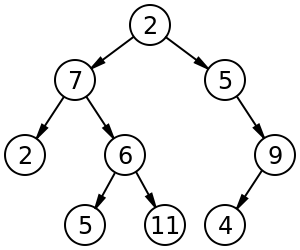
\includegraphics[width = 5cm]{Binary_tree.png}
		\caption{Primer dvojiškega drevesa.}
		\label{fig:drevo}
	\end{figure}
	
	\emph{Globina} drevesa je dolžina najdaljše poti od korena do (poljubnega) lista. Drevo na sliki ima globino $4$ (obstajajo tri različne poti, ki realizirajo to globino). Globina praznega drevesa je 0.  
	\emph{Obrnjeno drevo} dobimo iz dvojiškega drevesa, če vsakemu vozlišču zamenjamo levega in desnega otroka. 
	\begin{enumerate}
		\item Narišite obrnjeno drevo od drevesa na sliki.
		\item Z indukcijo dokažite, da je globina obrnjenega drevesa enaka globini prvotnega drevesa. 
	\end{enumerate}
\end{vaja}

\end{document}